\subsection{Quantum Computing Benchmarks (QML)}
{{\footnotesize
\noindent A suite of benchmarks evaluating quantum hardware and algorithms on tasks such as state 
preparation, circuit optimization, and error correction across multiple platforms.


\begin{description}[labelwidth=4cm, labelsep=1em, leftmargin=4cm, itemsep=0.1em, parsep=0em]
  \item[date:] 2022-02-22
  \item[version:] 1
  \item[last\_updated:] 2022-02-22
  \item[expired:] false
  \item[valid:] yes
  \item[valid\_date:] 2022-02-22
  \item[url:] \href{https://github.com/XanaduAI/qml-benchmarks}{https://github.com/XanaduAI/qml-benchmarks}
  \item[doi:] 10.48550/arXiv.2403.07059
  \item[domain:]
    - Computational Science \& AI
  \item[focus:] Quantum algorithm performance evaluation
  \item[keywords:]
    - quantum circuits
    - state preparation
    - error correction
  \item[licensing:] Apache-2.0
  \item[task\_types:]
    - Circuit benchmarking
    - State classification
  \item[ai\_capability\_measured:]
    - Quantum algorithm performance and fidelity
  \item[metrics:]
    - Fidelity
    - Success probability
  \item[models:]
    - IBM Q
    - IonQ
    - AQT@LBNL
  \item[ml\_motif:]
    - Classification
  \item[type:] Benchmark
  \item[ml\_task:]
    - Supervised Learning
  \item[solutions:] Varies per benchmark
  \item[notes:] Hardware-agnostic, application-level metrics. The citation may not be correct.
  \item[contact.name:] Xanadu AI
  \item[contact.email:] support@xanadu.ai
  \item[datasets.links.name:] PennyLane QML Benchmarks Datasets
  \item[datasets.links.url:] \href{https://pennylane.ai/datasets/collection/qml-benchmarks}{https://pennylane.ai/datasets/collection/qml-benchmarks}
  \item[results.links.name:] QML Benchmarks GitHub Repository (Results section)
  \item[results.links.url:] \href{https://github.com/XanaduAI/qml-benchmarks\#results-and-leaderboards}{https://github.com/XanaduAI/qml-benchmarks\#results-and-leaderboards}
  \item[fair.reproducible:] Yes
  \item[fair.benchmark\_ready:] Yes
  \item[id:] quantum\_computing\_benchmarks\_qml
  \item[Citations:] \cite{bowles2024betterclassicalsubtleart}
\end{description}

{\bf Ratings:} ~ \\

\begin{tabular}{p{0.15\textwidth} p{0.07\textwidth} p{0.7\textwidth}}
\hline
Rating & Value & Reason \\
\hline
dataset & 4 & Datasets are accessible, but not split.
 \\
documentation & 5 & Paper is available with all required information. 
 \\
metrics & 3 & Partially defined, somewhat inferrable metrics. Unknown whether a system's performance is captured.
 \\
reference\_solution & 0 & Not provided
 \\
software & 4 & Software is built upon multiple common frameworks for simulation, training, and benchmarking workflows.
 \\
specification & 3 & No system constraints. Task clarity and dataset format are not clearly specified.
 \\
\hline
\end{tabular}

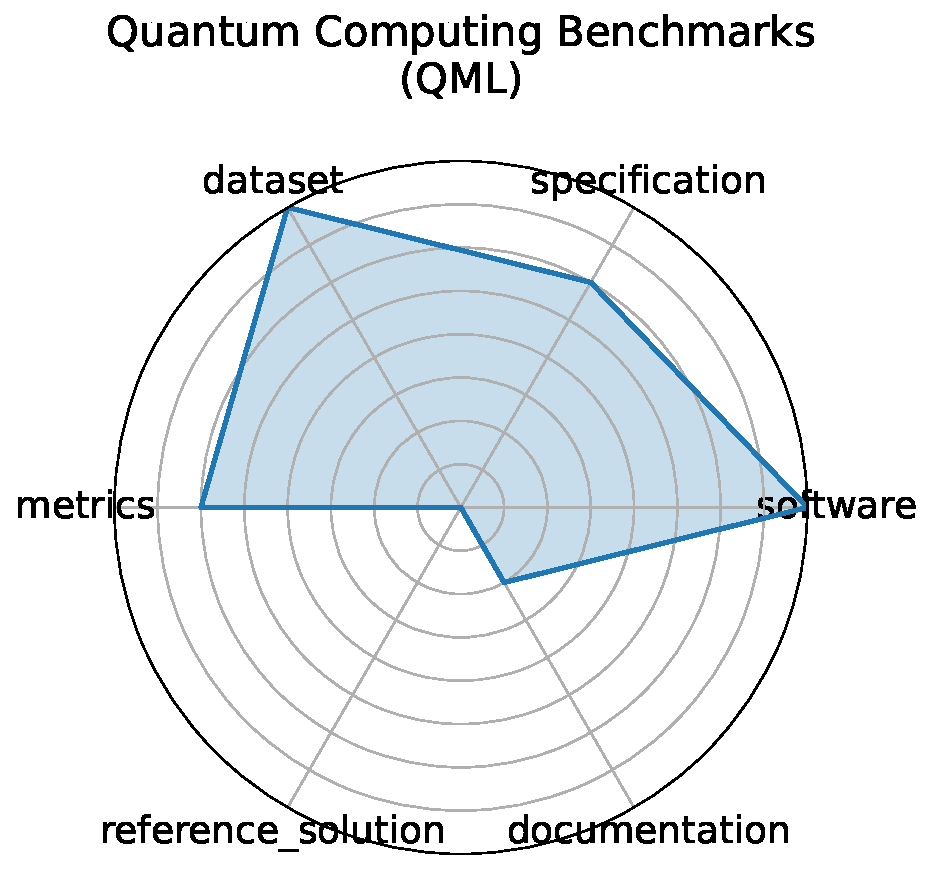
\includegraphics[width=0.2\textwidth]{quantum_computing_benchmarks_qml_radar.pdf}
}}
\clearpage